\documentclass[14pt,aspectratio=169]{beamer}

% Assets
\usepackage[czech]{babel}				% Jazyk
\usepackage[a-2u]{pdfx}					% Kopírování z pdfka
\usepackage{tikz}						% Schémata automatů
\usepackage{csquotes}					% české uvozovky
\usepackage{enumerate}					% enumerate environment
\usepackage{indentfirst}
\usepackage{mathtools}
\usepackage{pifont}
\usepackage{xcolor}
\usepackage{enumitem,xcolor}
\usepackage{amsmath}
\usepackage[utf8]{inputenc}

\usepackage{listings}                   % Úryvky z kódu (C#)
\lstset{language=[Sharp]C, frame=lr}
% Beamer theme
\usetheme{Boadilla}
\setbeamertemplate{frame numbering}[fraction]
\usecolortheme[named=black]{structure}
\setbeamertemplate{navigation symbols}{}
\setbeamerfont{title}{series=\bfseries,parent=structure}
\setbeamerfont{frametitle}{series=\bfseries,parent=structure}
\usefonttheme[onlymath]{serif}
\urlstyle{same}

% Dark theme
\setbeamercolor{frametitle}{fg=white}
\setbeamercolor{title}{fg=white}
\setbeamercolor{background canvas}{bg=black}
\setbeamercolor{normal text}{fg=white}

\defbeamertemplate*{title page}{customized}[1][]
{ 
  \usebeamerfont*{title}\inserttitle\par
  \bigskip
  \usebeamerfont*{subtitle}\textit{\insertsubtitle}\par
  \bigskip \bigskip \bigskip \bigskip 
  \usebeamerfont{author}\insertauthor\par
  \usebeamerfont{institute}Kabinet \office\\\url{weber3@spsejecna.cz}\bigskip
}
% Enumerate
%\setlist[enumerate]{topsep=0pt,itemsep=-1ex,partopsep=1ex,parsep=1ex,label=(\arabic*)}

\MakeOuterQuote{"}

% Colors
\definecolor{lightblue}{HTML}{009AD4}
\definecolor{darkgreen}{HTML}{0D7103}
\definecolor{lightgreen}{HTML}{68FF00}
\definecolor{darkred}{HTML}{AF0B0B}
\definecolor{lightred}{HTML}{FF5100}
\definecolor{orange}{HTML}{FFE000}
\definecolor{codeblue}{HTML}{FF0055}
\definecolor{codegreen}{rgb}{0,0.6,0}
\definecolor{codegray}{rgb}{0.5,0.5,0.5}
\definecolor{codebeige}{HTML}{D4A000}
\definecolor{backcolour}{rgb}{0.95,0.95,0.92}

\newcommand{\markred}[1]{\textcolor{lightred}{#1}}
\newcommand{\markgreen}[1]{\textcolor{lightgreen}{#1}}
\newcommand{\markorange}[1]{\textcolor{orange}{#1}}
\newcommand{\markblue}[1]{\textcolor{lightblue}{#1}}

% Inline images
\newcommand{\inlineimgscale}{1.1}

% X and check mark
\newcommand{\cmark}{\markgreen{\ding{51}}}
\newcommand{\xmark}{\markred{\ding{55}}}

% Redefinions
\renewcommand{\implies}{\Rightarrow}
\renewcommand{\impliedby}{\Leftarrow}

% Math
\newcommand{\R}{\mathbb{R}}
\newcommand{\C}{\mathbb{C}}
\newcommand{\N}{\mathbb{N}}
\newcommand{\Z}{\mathbb{Z}}
\newcommand{\Q}{\mathbb{Q}}

% Code
\lstdefinestyle{clang}{
    basicstyle=\small\ttfamily\color{white},
    language=C,
    keywordstyle=\color{codeblue},
    commentstyle=\color{codegreen},
    numberstyle=\tiny\color{codegray},
    stringstyle=\color{codebeige},
    breakatwhitespace=false,
    breaklines=true,
    captionpos=b,
    keepspaces=true,
    numbersep=5pt,
    showspaces=false,
    showstringspaces=false,
    showtabs=false,
    morekeywords={void,int,double,float,unsigned,if,else,\#include}
    tabsize=0.5
}
\lstset{escapeinside={(*}{*)},style=clang}

\newcommand{\hlcode}[1]{\colorbox{red}{#1}}

% Title page
\title{Adresy a ukazatele v C}
\subtitle{Informační a komunikační technologie}
\author{David Weber}
\def\office{K13}
\def\email{weber3@spsejecna.cz}

\begin{document}

    % Itemize
    \setlist[itemize]{label=\textcolor{white}{\textbullet}}

    % Slides
    \begin{frame}
        \titlepage
    \end{frame}

    \begin{frame}[t]{Připomenutí}
        \begin{itemize}
            \item Jaký je rozdíl mezi \emph{adresou} a \emph{hodnotou} proměnné?
            \begin{itemize}
                \item \textbf{Hodnota} -- hodnota uložená v paměťové buňce proměnné
                \item \textbf{Adresa} -- číslo paměťové buňky proměnné
            \end{itemize}
            \item Pro výpis jsme používali znak \texttt{\&}.
        \end{itemize}
        \begin{figure}
            \centering
            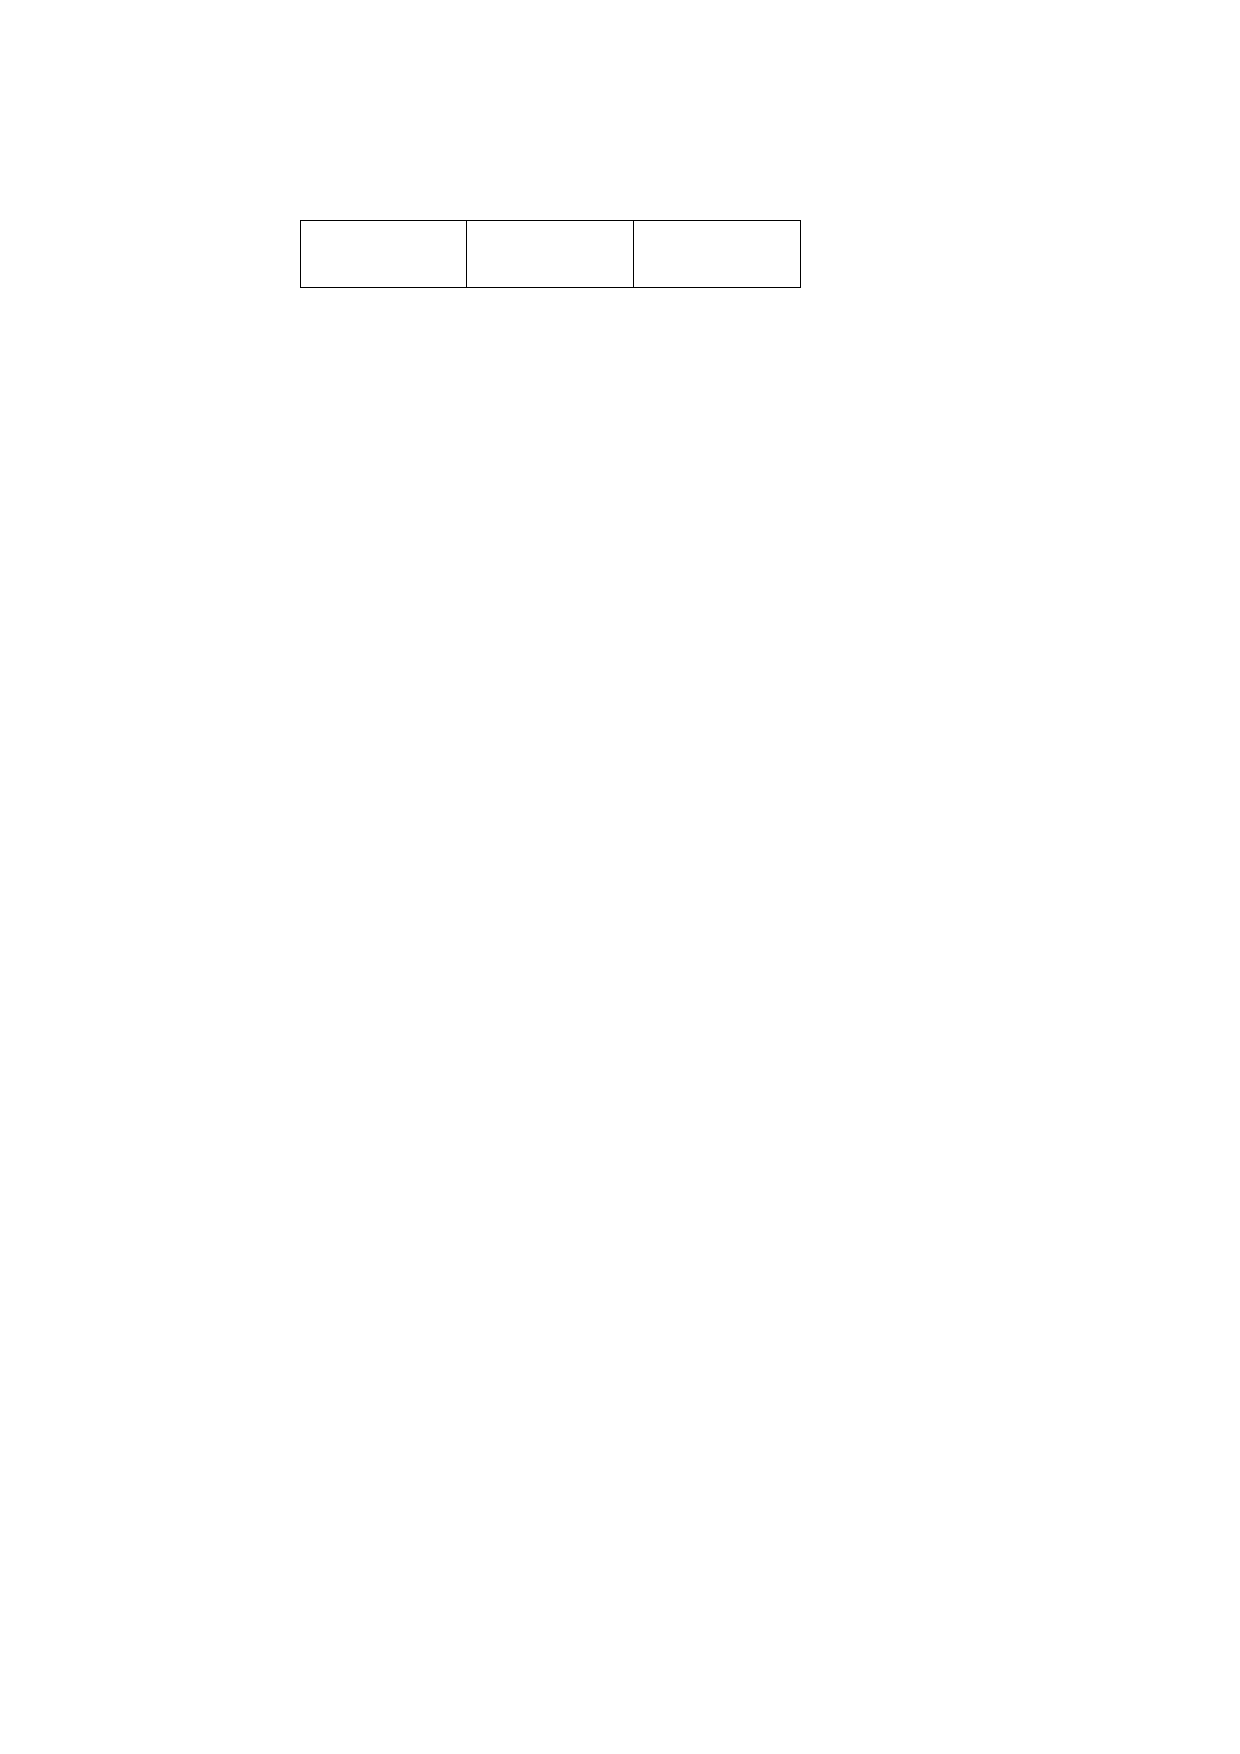
\includegraphics{images/memory_variable.pdf}
        \end{figure}
        \begin{itemize}
            \item Předpona \texttt{0x} značí číslo zapsané \textbf{hexadecimálně} (v C, ale i jiných jazycích).
        \end{itemize}
    \end{frame}

    \begin{frame}[t,fragile]{Příklad na úvod I}
        Mějme program obsahující funkci pro prohození hodnot proměnných \texttt{u} a \texttt{v}.
        \begin{lstlisting}
void swap(int u, int v) {
    int temp = u;
    u = v;
    v = temp;
}
int main(void) {
    int a = 5;
    int b = 10;
    swap(a, b);
    printf("Hodnoty a, b: %d, %d", a, b);
    return 0;
}
        \end{lstlisting}
    \end{frame}

    \begin{frame}[t]{Příklad na úvod II}
        Jaký bude výstup předešlého programu?
        \begin{enumerate}[label=(\alph*)]
            \item \texttt{Hodnoty a, b: 5, 10}
            \only<1>{\item \texttt{Hodnoty a, b: 10, 5}}
            \only<2->{\item \markgreen{\texttt{Hodnoty a, b: 10, 5}}}
        \end{enumerate}
        \only<3->{\markred{$\implies$ nijak jsme si nepomohli \emoji{crying-face}}}
    \end{frame}

    \begin{frame}[t]{V čem je problém?}
        \begin{itemize}
            \item Parametry funkci předáváme tzv. \textbf{hodnotou}.
            \begin{itemize}
                \item Hodnoty proměnných \texttt{a} a \texttt{b} jsou zkopírovány a při volání funkce \texttt{swap} jsou nově \emph{na zásobníku} deklarovány proměnné \texttt{u} ~a \texttt{v}.
                \item \markred{$\implies$ funkce v konečném důsledku prohodí hodnoty proměnných \texttt{u} a \texttt{v}, nikoliv \texttt{a} a \texttt{b}}
            \end{itemize}
            \item \markgreen{$\implies$ mohli bychom vyřešit předáním ``odkazů'' na původní proměnné.}
        \end{itemize}
    \end{frame}

    \begin{frame}[t,fragile]{Ukazatel (pointer) I}
        \begin{itemize}
            \item \textbf{Datový typ} uchovávající adresu v paměti \textbf{určitého datového typu} (existují i generické ukazatele, ale ty nebudeme řešit \emoji{slightly-smiling-face}).
            \item Při deklaraci je třeba uvést datový typ hodnoty (tím kompilátoru říkáme, jak se má interpretovat místo v paměti, kam ukazuje ), jejíž adresu ukazatel uchovává, a znak \texttt{*} (pro odlišení od deklarace standardní proměnné).
            \item Jedná se vždy o \textbf{kladné celé číslo} (formátová specifikace \texttt{\%p}).
            \begin{lstlisting}
int main(void) {
    int x = 50;
    int *px = &x;
    printf("Hodnota x: %d\nAdresa x: %p", x, px);
    return 0;
}
            \end{lstlisting}
        \end{itemize}
    \end{frame}

    \begin{frame}{Ukazatel (pointer) II}
        \begin{figure}
            \centering
            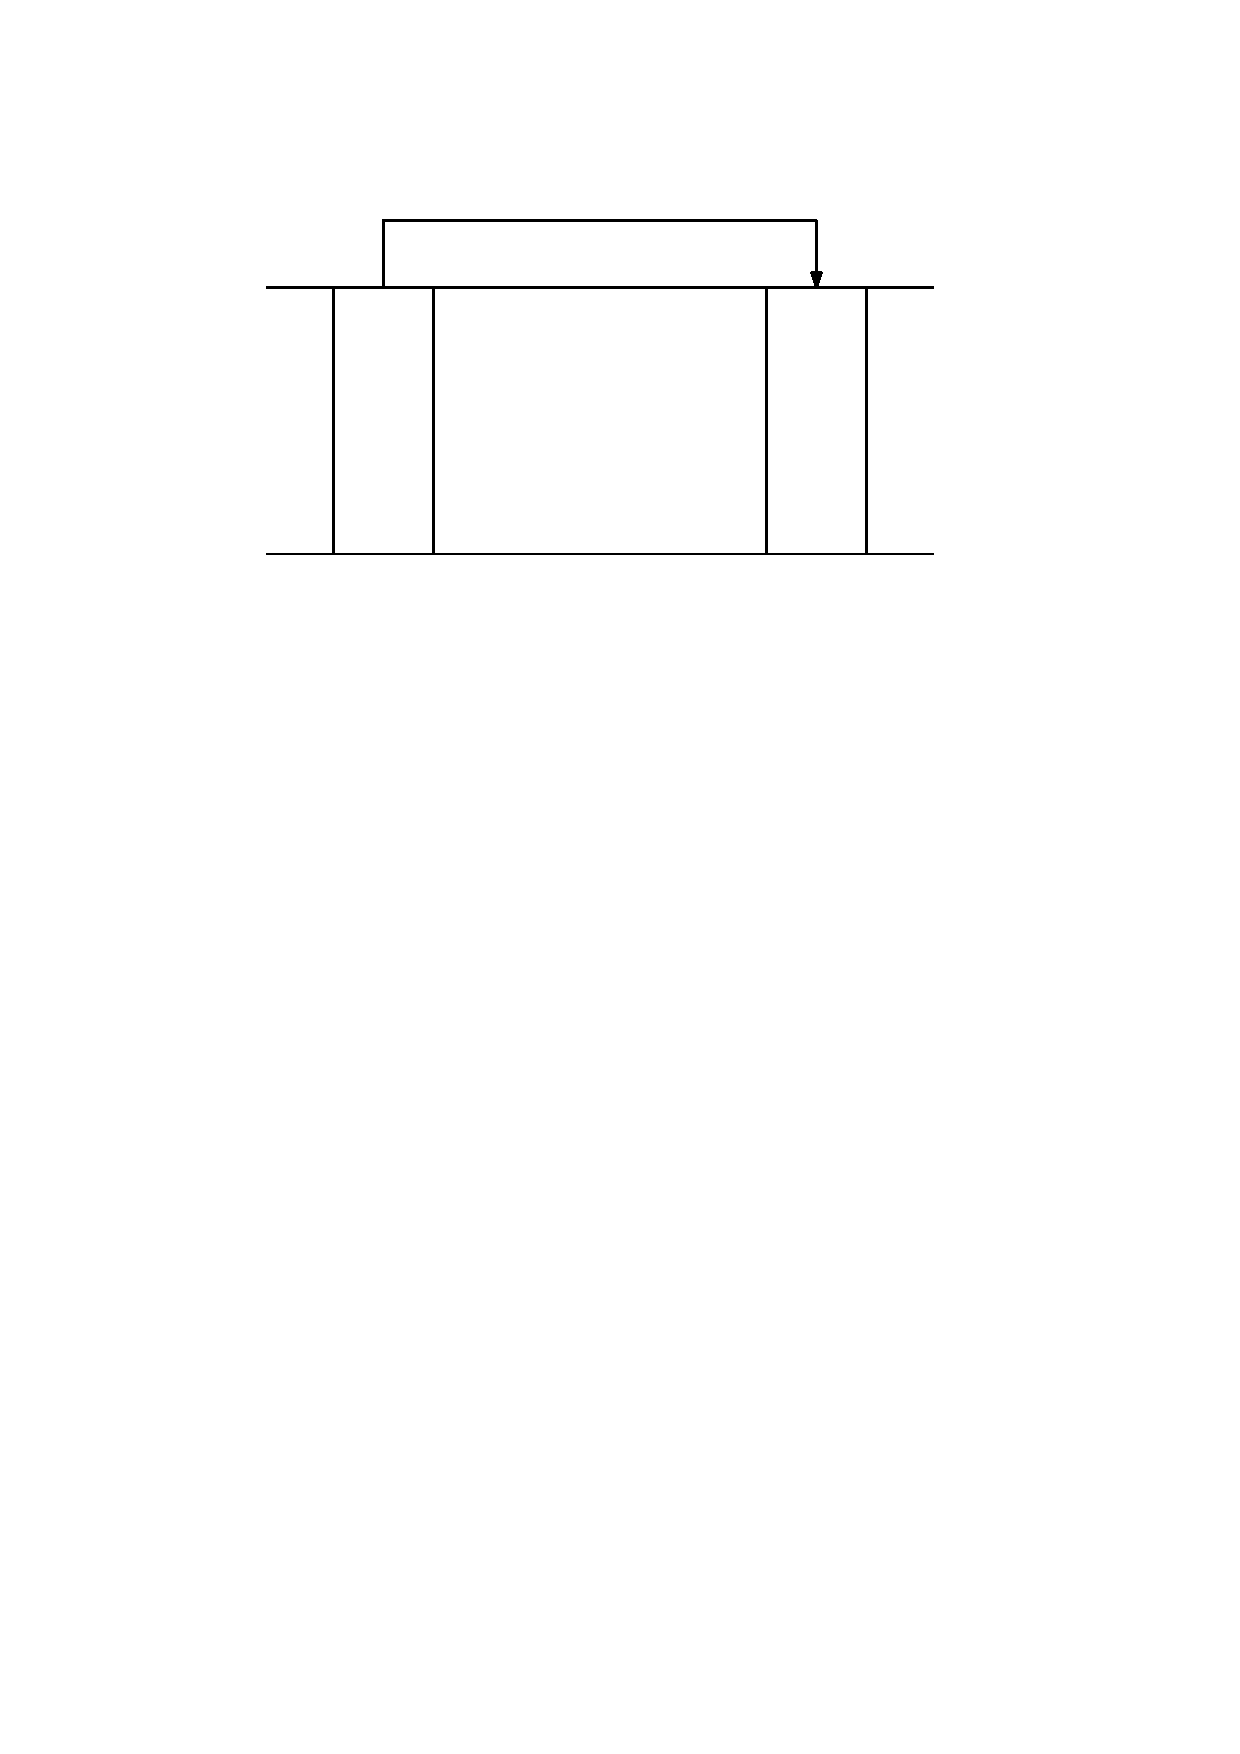
\includegraphics[scale=.75]{images/pointer_to_variable.pdf}
        \end{figure}
    \end{frame}

    \begin{frame}[t,fragile]{Dereference}
        \begin{itemize}
            \item Ekvivalentně lze deklaraci ukazatele zápisem \texttt{int* p} (mezera mezi \texttt{*} a \texttt{p}).
            \item Co když máme adresu, ale ne samotnou proměnnou? $\implies$ \markgreen{využijeme tzv. \textbf{operátor dereference} \texttt{*}.}
            \begin{itemize}
                \item Umožňuje nám odkázat se přímo na \textbf{hodnotu} v paměťové buňce ležící na \textbf{adrese ukazatele}.
            \end{itemize}
            \begin{lstlisting}
int main(void) {
    int i = 50;
    int *p = &i;
    *p = 100;           // same as i = 100;
    printf("%d", i);    // prints out "100"
    return 0;
}
            \end{lstlisting}
        \end{itemize}
    \end{frame}

    \begin{frame}[t,fragile]{Původní problém}
        Jak bychom měli upravit původní program, aby fungoval?
        \begin{lstlisting}
void swap(int u, int v) {
    int temp = u;
    u = v;
    v = temp;
}
int main(void) {
    int a = 5;
    int b = 10;
    swap(a, b);
    printf("Hodnoty a, b: %d, %d", a, b);
    return 0;
}
        \end{lstlisting}
    \end{frame}

    \begin{frame}[t,fragile]{Řešení}
        \begin{itemize}
            \item Je potřeba předat funkci \texttt{swap} adresu proměnných \texttt{a} a \texttt{b} (tzv. předání \textbf{referencí}).
            \item Uvnitř těla funkce pak provedeme dereferenci ukazatelů.
            \begin{lstlisting}
void swap(int *u, int *v) {
    int temp = *u;
    *u = *v;
    *v = temp;
}
            \end{lstlisting}
        \end{itemize}
    \end{frame}

    \begin{frame}[t,fragile]{Pole a ukazatele I}
        \begin{itemize}
            \item Již jsme si zmínili, že pole je struktura uchovávající více prvků \textbf{stejného datového typu}.
            \item Na jednotlivé buňky pole jsme se při načítání hodnot z konzole odkazovali pomocí jejich adresy v paměti.
            \begin{lstlisting}
int arr[10];
for (int i = 0; i < 10; i++) {
    if (scanf("%d", &arr[i]) < 1) {
        printf("ERROR.");
        return -1;
    }
}
            \end{lstlisting}
        \end{itemize}
    \end{frame}

    \begin{frame}[t,fragile]{Pole a ukazatele II}
        \begin{itemize}
            \item Samotný "výraz" \texttt{arr} jsme používali (zatím) vždy pouze s indexem při odkazování na konkrétní prvek (např. \texttt{arr[i]}).
            \item Co ovšem představuje sám o sobě? \markorange{$\implies$ ukazatel na počátek pole! (Tzn. prvek na nultém indexu.)}
            \begin{lstlisting}
int main() {
    int arr[] = { 1, 2, 3 };

    // arr and &arr[0] are identical
    printf("%p %p", arr, &arr[0]);
    return 0;
}
            \end{lstlisting}
        \end{itemize}
    \end{frame}

    \begin{frame}[fragile]{Příklad (hledání prvku v poli) I}
        \begin{lstlisting}
unsigned int getElementIndex(int arr[], int size, int element) {
    for (int i = 0; i < size; i++) {
        if (arr[i] == element)
            return i;
    }
    return -1;
}
        \end{lstlisting}
    \end{frame}

    \begin{frame}[t]{Příklad (hledání prvku v poli) II}
        \begin{itemize}
            \item Funkce \texttt{getElementIndex} přijímá jako parametr pole \texttt{arr}, které je předáváno \textbf{referencí}.
            \item \markred{Předávání hodnotou by mohl být problém, neboť pro velké struktury (řádově např. statisíce prvků) bychom museli všechny prvky kopírovat.}
            \item Lze též psát \texttt{int* arr}.
        \end{itemize}
    \end{frame}

    \begin{frame}[t,fragile]{Pole a ukazatele III}
        \begin{lstlisting}
int main(void) {
    int arr[5];
    int *p = arr;
    printf("%p, %p", sizeof(arr), sizeof(p));
    return 0;
}
        \end{lstlisting}
        \begin{itemize}
            \item Je dobré si uvědomit, že byť \texttt{arr} ukazuje na počátek pole, přesto je zde rozdíl oproti ukazateli \texttt{p}.
            \item \markred{$\implies$ \texttt{sizeof(arr)} vypíše velikost pole \texttt{arr} v bytech, zatímco \texttt{sizeof(p)} vypíše velikost ukazatele \texttt{p}!}
        \end{itemize}
    \end{frame}

    \begin{frame}[t]{Aritmetika s ukazateli I}
        \begin{itemize}
            \item Ukazatele jsou číselné proměnné $\implies$ lze s nimi manipulovat pomocí $+,\,-$.
            \item Nelze např. sčítat/odčítat dvojici ukazatelů, tj. \texttt{p1 + p2}
            \item Lze psát např. \texttt{p++}, \texttt{p--}, \texttt{p -= 4}, \dots
            \item \markorange{\textbf{Inkrementace}, resp. \textbf{dekrementace} probíhá vždy o násobky velikosti datového typu, na který ukazatel ukazuje (nikoliv přímo o danou hodnotu)!}
        \end{itemize}
    \end{frame}

    \begin{frame}{Aritmetika s ukazateli II}
        \begin{figure}
            \centering
            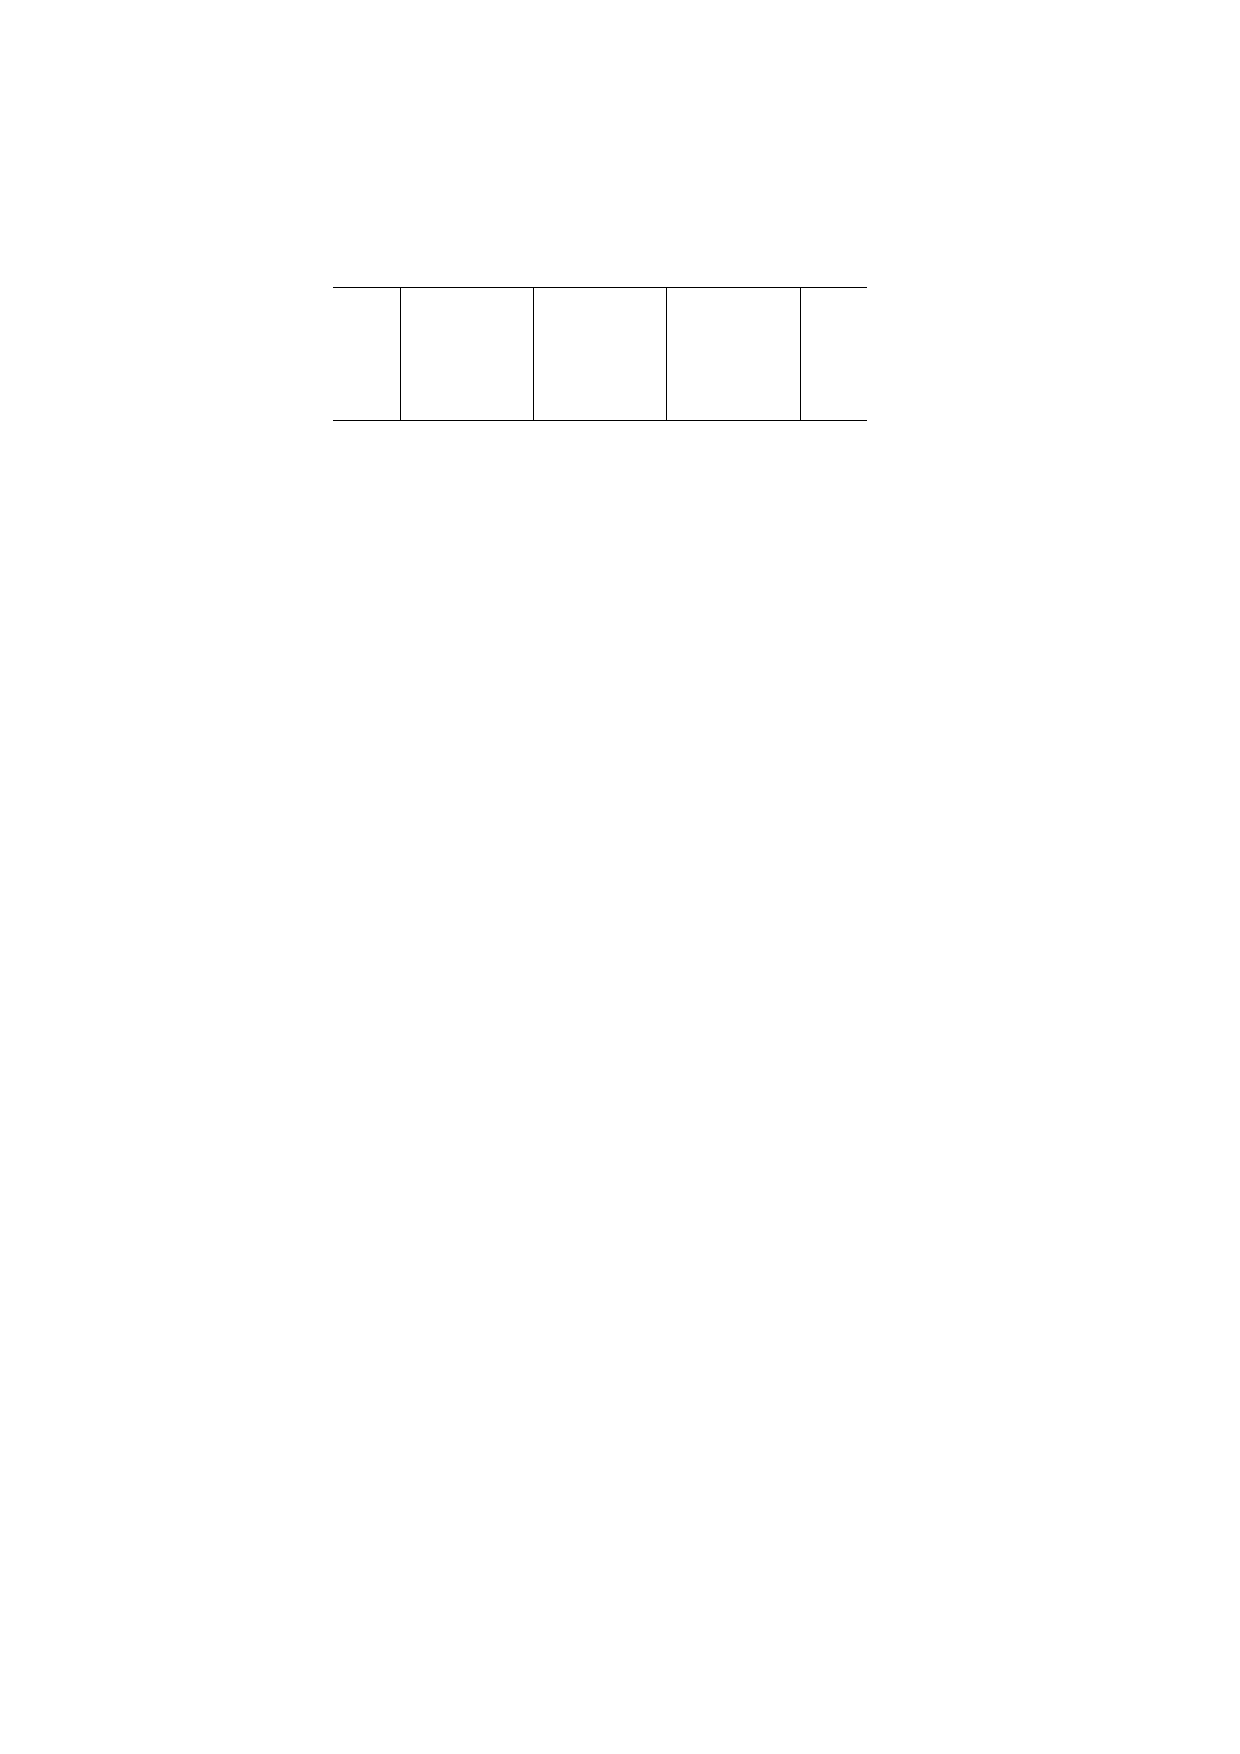
\includegraphics{images/pointer_arith.pdf}
        \end{figure}
    \end{frame}

    \begin{frame}[fragile]{Příklad}
        Výpis prvků pole.
        \begin{lstlisting}
void printArray(int arr[], unsigned int size) {
    int *p = arr;       // First element address
    for (int i = 0; i < size; i++) {
        printf("%d", *(p+i));
    }
}
        \end{lstlisting}
    \end{frame}

    \begin{frame}{Otázky?}
        \begin{figure}
            \centering
            
\includegraphics[scale=.4]{images/discussion_inverted.png}
        \end{figure}
    \end{frame}

\end{document}